\section{Vulnerability: Tokens are 1-10 and don't expire}
\label{sec:background}
\textbf{Description:} The access tokens on the website have 2 key issues. Firstly there are only ten eleven tokens availabe (0 through to 10). Secondly the tokens have no expiry
date and as such if a hacker were to gain access to a token through for example Javascript injection as seen in vulnerability 3, he could use it to keep permanent access to a
user's account even if they changed their password, regardless of how complex the password hashing was made. This of course is a serious security flaw and needs to be addressed.
By only having 11 tokens this flaw is made worse since an attacker would only need to try 11 tokens in order to get access. \\ \\
\textbf{Testing the Vulnerability:} To do this I logged in as \textit{hacker@wondoughbank.com} and displayed the transactions. After my fix to the login issue in the previous
vulnerability the result was identical to figure \ref{figvun6}. I then went into the developer options on my browser to display the cookies:
\begin{figure}[h]
    \centering
    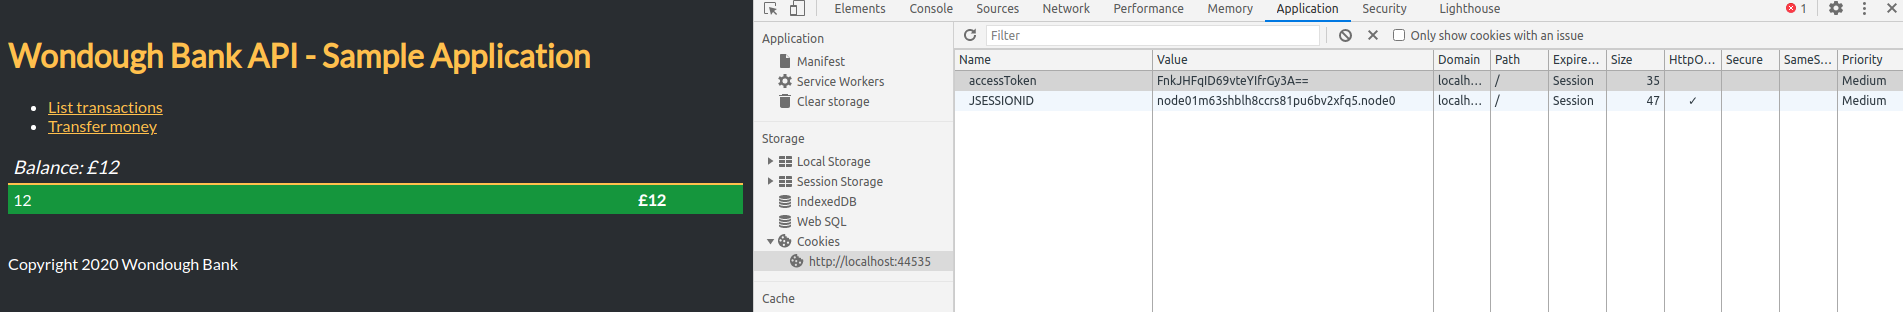
\includegraphics[width=1\textwidth]{figs/7.1.png}
    \caption{The token visible in the cookies of my session}
    \label{7.1}
\end{figure}\\
From here I was able to change the token to one associated with user 0 (from \textit{jxTkX87qFnpaNt7dS+olQw==} to \textit{jxTkX87qFnpaNt7dS+olQw==}):
\begin{figure}[h]
    \centering
    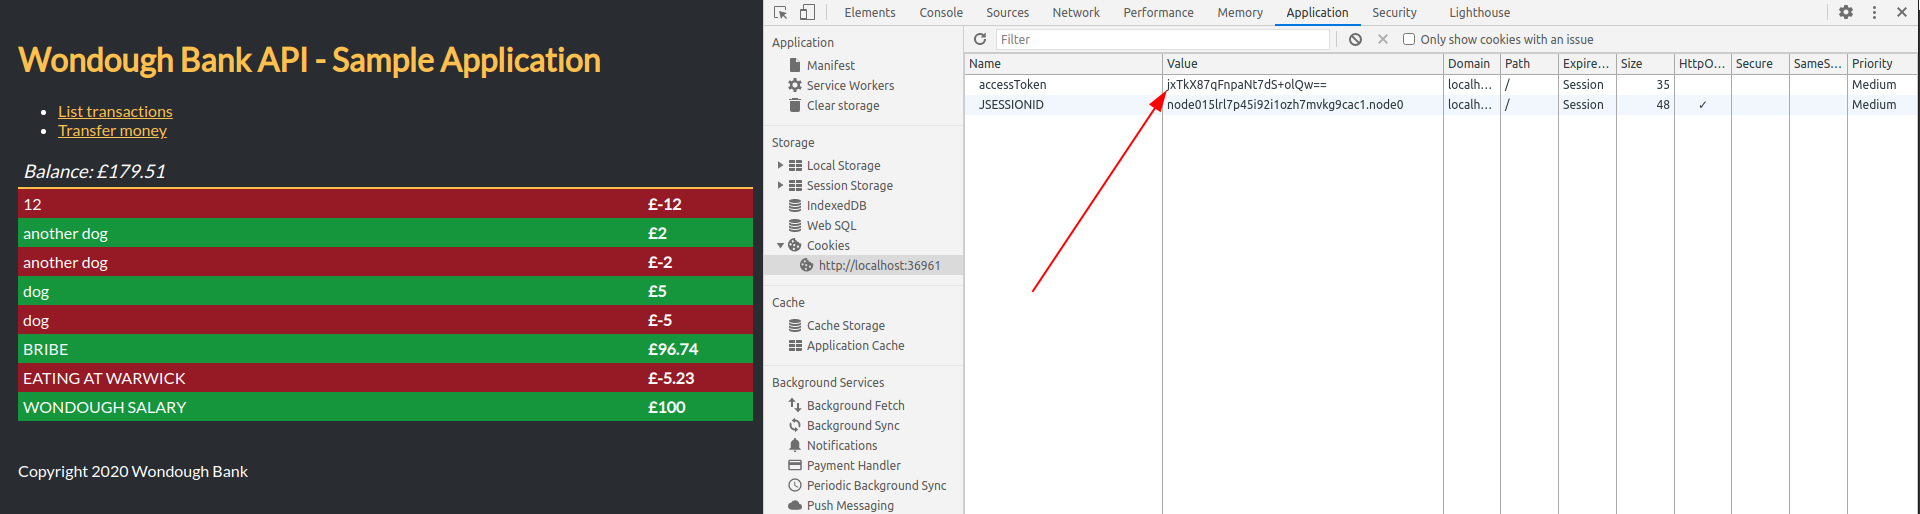
\includegraphics[width=1\textwidth]{figs/7.2.png}
    \caption{By editing the token I gain access to the intern's account}
    \label{7.2}
\end{figure}\\

\\ \\
\textbf{Mitigation:} The first issue of the 0-10 occurs in \verb|dbConnection| where the following code is used to create the tokens id:\\
\begin{minted}{java}
app.setRequestToken(Integer.toString(this.largestRequestToken(), 10));
app.setAccessToken(Integer.toString(this.largestAccessToken(), 10));
\end{minted}
I have therefore chosen to use the salt generation as the token since this is unique each time and much more complex. It also means that the issue of the access and request token
being the same solved.
\begin{minted}{java}
String salt;
salt = Program.getInstance().getSecurityConfiguration().generateSalt();
app.setRequestToken(salt);
salt = Program.getInstance().getSecurityConfiguration().generateSalt();
app.setAccessToken(salt);
\end{minted}